\chapter{Topics in String Theory}

These notes follow Leonard Susskind's ninth lecture in the supplementary Cosmology and Black Holes track, and are curated as companion notes by LazyingArt LLC. The lecture really begins before the formal lecture begins: a student asks how a cosmic horizon can possibly be hot, and Susskind turns that question into the organizing problem of the evening. The discussion then unfolds in a deliberate sequence. First comes the operational meaning of horizon temperature in the black-hole case, then the spacetime picture of emission and reabsorption near a stretched horizon, then the transfer of the same logic to de Sitter space, and finally the statistical mechanics of a finite-entropy causal patch, with recurrences, Boltzmann brains, eternal inflation, and the measure problem appearing as its long-time consequences.

\section{Horizons Are Always Hot}

A student asks for a mechanism, not a slogan: how is a cosmic horizon hot? Susskind's first answer is blunt, ``exactly the same as in the black hole,'' but he immediately sharpens that claim. The right starting point is not an abstract theorem but a real experiment. If one lowers a thermometer toward a horizon, the thermometer reads an ever larger temperature. In the lecture this is summarized by the near-horizon rule
\begin{equation}
T_{\text{local}}(d_{\text{hor}})\sim \frac{1}{2\pi\, d_{\text{hor}}},
\end{equation}
where \(d_{\text{hor}}\) is the proper distance to the horizon. Susskind presents this as a universal property of horizons: black-hole horizon, cosmic horizon, any horizon.

This immediately answers the student's first question, but it also creates the next one. If the near-horizon region is so hot, why is a distant observer not blasted by enormously energetic radiation? Susskind formulates this concretely. A huge hot wall would keep looking hot far away. Its high-frequency photons would still blind you. A black-hole horizon does not behave that way. Why not?

The answer is gravitational redshift. A photon emitted near the horizon loses energy as it climbs away. Susskind insists that for photons one should speak directly about energy rather than velocity. The energy falls during the outward trip, and so the observer at infinity sees not the enormous local temperature but the Hawking temperature,
\begin{equation}
T_H\sim \frac{1}{8\pi M},
\end{equation}
in natural units for a Schwarzschild black hole of mass \(M\).

This separation between the local temperature and the redshifted temperature is the first major conceptual step of the lecture. The horizon is locally extremely hot. The radiation detected far away is much colder. The larger the black hole, the smaller this asymptotic temperature. Susskind's explanation is again operational: the larger hole makes the escaping photon do more work on the way out, so the distant observer receives less energy.

The same point can be phrased in the language of typical quanta. For thermal radiation, the characteristic photon energy is of the same order as the temperature. Thus
\begin{equation}
E_{\gamma,\infty}\sim T_H\sim \frac{1}{M}.
\end{equation}
If one traces such a photon back inward and asks what energy it must have had when it emerged from the near-horizon region, one is led back to the same universal local scale \(1/(2\pi d_{\text{hor}})\). Susskind then pushes the argument one step further. The smallest meaningful distance to the horizon is of order the Planck length, so the emission should be thought of as originating in a very thin Planck-scale layer.

This is exactly where the lecture changes pictures. The thermodynamic story is not abandoned, but it is re-expressed geometrically.

\section{Quantum Fluctuations And The Stretched Horizon}

Susskind's next move is signaled explicitly in the lecture: ``there's another way to think about it.'' Instead of talking only about temperatures and redshifted photons, he wants a spacetime picture of what the horizon is doing.

The first part of that picture is still quasi-thermal. A thin Planck-scale layer near the horizon continuously emits and absorbs extremely energetic quanta. Most of them do not escape. Only a tiny escape cone of almost radially outward directions allows a photon to get away; quanta emitted at generic angles fall back. The near-horizon region is therefore not a calm surface but a violent bath of outgoing and ingoing energetic quanta. Those quanta collide, produce pairs and other excitations, and maintain a thin shell of very hot material.

\begin{figure}
\centering

\includegraphics[width=0.46\textwidth]{lecture_09_figure_02.png}
\caption{Initial black-hole causal scaffold.}
\end{figure}

\begin{figure}
\centering

\begin{tikzpicture}[scale=1.0]
\draw[thick] (-2.2,2.2) -- (0,0) -- (2.2,-2.2);
\draw[thick] (-2.2,-2.2) -- (0,0) -- (2.2,2.2);
\end{tikzpicture}
\caption{Clean redraw of the causal scaffold that anchors the black-hole discussion.}
\end{figure}

He then recasts the same story in a more geometric language. The lecture uses the rough metaphor of quantum fluctuations as virtual closed loops. Away from the horizon such loops are too short-lived to be directly real. Near the horizon, however, one can have fluctuations that sit partly on one side and partly on the other. To the outside observer such a fluctuation looks like emission from the horizon followed by reabsorption. Hawking radiation is the tiny fraction of these processes that does not fall back in.

This is why the horizon appears thermally active. The horizon does not create particles by hand. Rather, the horizon turns otherwise virtual near-horizon fluctuations into real thermal phenomena for the relevant observer.

\begin{figure}
\centering

\includegraphics[width=0.46\textwidth]{lecture_09_figure_03.png}
\caption{Horizon redrawn as a vertical boundary.}
\end{figure}

\begin{figure}
\centering
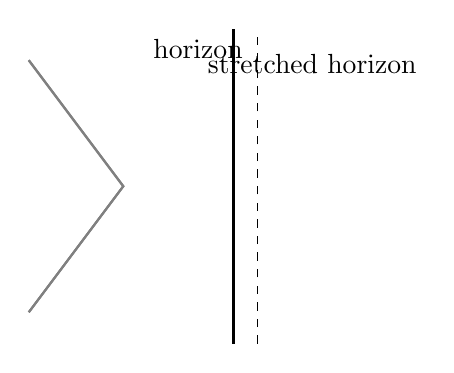
\begin{tikzpicture}[scale=1.0]
\draw[gray,thick] (-2.0,1.6) -- (-0.8,0) -- (-2.0,-1.6);
\draw[gray,thick] (-2.0,-1.6) -- (-0.8,0) -- (-2.0,1.6);
\draw[thick] (0.6,-2.0) -- (0.6,2.0);
\draw[dashed] (0.9,-2.0) -- (0.9,2.0);
\node at (0.15,1.75) {horizon};
\node at (1.6,1.55) {stretched horizon};
\end{tikzpicture}
\caption{A cleaned reconstruction of the lecture's alternate picture: a horizon drawn as a vertical boundary, together with a nearby stretched horizon one Planck length away.}
\end{figure}

The stretched horizon is introduced at precisely this point. The exact classical horizon should not be trusted at arbitrarily fine distance scales. Quantum fluctuations of matter and geometry smear it. So Susskind replaces the exact horizon by a nearby timelike surface, roughly one Planck length away. The gain is conceptual as much as technical: the relevant fluctuations now occur at finite exterior time rather than being banished to a formal \(t=\infty\).

This completes the black-hole warm-up. The point is not that black holes are special. The point is that the same horizon logic should apply to cosmic horizons as well.

\section{De Sitter Geometry From Expanding Coordinates To Causal Diagrams}

The lecture now pivots, using Susskind's own phrase, to ``cosmic horizons in the same vein.'' He begins with de Sitter space in the flat slicing,
\begin{equation}
ds^2=-dt^2+e^{2Ht}\,d\mathbf{x}^2,
\qquad
d\mathbf{x}^2=dx^2+dy^2+dz^2.
\end{equation}
Here \(H\) is the de Sitter Hubble constant, and a fixed coordinate interval corresponds to a growing physical distance,
\begin{equation}
\Delta x_{\text{phys}}(t)=e^{Ht}\,\Delta x.
\end{equation}
That is the exponential expansion of space.

Susskind then introduces a coordinate trick whose purpose is purely geometric: future infinity should be brought onto the blackboard so that one can reason about causality. In the transcript he corrects the transformation in real time, so the clean presentation is the standard conformal-time reconstruction
\begin{equation}
\eta=-\frac{1}{H}e^{-Ht},
\qquad
t\to +\infty \Longrightarrow \eta\to 0^-.
\end{equation}
The metric becomes
\begin{equation}
ds^2=\frac{1}{H^2\eta^2}\left(-d\eta^2+d\mathbf{x}^2\right).
\end{equation}
The lecture's real point is immediate. Since the conformal factor does not affect null directions, radial light rays satisfy
\begin{equation}
ds^2=0
\qquad\Longrightarrow\qquad
d\eta=\pm dx,
\end{equation}
so light rays run at \(45^\circ\).

This is why Susskind wants these coordinates. They make it visually obvious who can communicate with whom. We are to imagine, as he does in the lecture, an idealized observer who lives forever. The observer's worldline extends upward toward future infinity, and the physically accessible region is the backward light cone of that worldline.

\begin{figure}
\centering
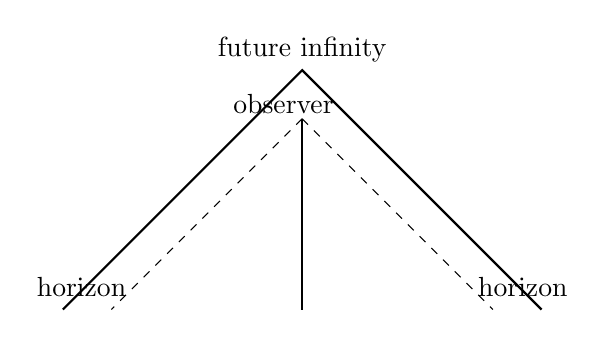
\begin{tikzpicture}[scale=0.95]
\draw[thick] (-3.2,0) -- (0,3.2) -- (3.2,0);
\draw[thick] (0,0) -- (0,2.55);
\draw[dashed] (0,2.55) -- (-2.55,0);
\draw[dashed] (0,2.55) -- (2.55,0);
\node at (-0.25,2.75) {observer};
\node at (0,3.48) {future infinity};
\node at (-2.95,0.3) {horizon};
\node at (2.95,0.3) {horizon};
\end{tikzpicture}
\caption{Transcript-led conformal reconstruction of a de Sitter observer and the backward light cone that defines the accessible spacetime region.}
\end{figure}

Susskind emphasizes that this narrowing to one observer is not a small matter. Different observers have different backward light cones and only partial overlap. The lecture temporarily suppresses that complication in order to focus on one causal patch at a time.

\section{The Observer's Horizon And The Static Patch}

At first sight the conformal diagram suggests that the observer's horizon might be changing with time. The horizontal width of the backward light cone becomes smaller as one moves upward. Susskind interrupts that impression with one of his characteristic ``simple exercises.'' It is the bridge between the conformal diagram and the static patch.

Take two points on a constant-\(\eta\) slice, one at the observer and one on the horizon. There is no time separation between them, so the interval is purely spatial. From the conformal metric,
\begin{equation}
D^2=\frac{(\Delta x)^2}{H^2\eta^2}.
\end{equation}
Now use the geometry of the diagram itself. The horizon line is at \(45^\circ\), so on the slice under consideration the horizontal distance to the horizon equals the vertical conformal-time distance:
\begin{equation}
\Delta x=|\eta|.
\end{equation}
Substitution gives
\begin{align}
D^2&=\frac{\eta^2}{H^2\eta^2}=\frac{1}{H^2},\\
D_{\text{hor}}&=\frac{1}{H}.
\end{align}
The important point is not the algebra but the invariance. The answer does not depend on \(\eta\). The physical distance to the horizon is always the same.

This is exactly the moment in the lecture when Susskind says that one should now expect a coordinate system adapted to the observer in which the geometry looks time independent. He does not derive it in detail. He simply writes the answer, correcting a sign slip as he goes:
\begin{equation}
ds^2=-(1-H^2r^2)\,dt^2+\frac{dr^2}{1-H^2r^2}+r^2\,d\Omega_2^2.
\end{equation}
This is the static patch, or causal patch, and it covers the region
\begin{equation}
0\le r\le \frac{1}{H}.
\end{equation}

\begin{figure}
\centering

\includegraphics[width=0.72\textwidth]{lecture_09_figure_04.png}
\caption{Static-patch metric and de Sitter horizon radius.}
\end{figure}

The coefficients of this metric depend on \(r\) but not on \(t\). That is the mathematical statement that the observer's environment is stationary. If the observer repeats the same local experiment later, the answer is the same. Objects released from rest will still accelerate away from one another, but the same experiment performed later reproduces the same result. This is Susskind's operational meaning of ``static.''

The comparison with Schwarzschild is immediate. In the black-hole case the key factor is
\begin{equation}
1-\frac{2MG}{r},
\end{equation}
while in the de Sitter static patch it is
\begin{equation}
1-H^2r^2.
\end{equation}
In both geometries the horizon sits where this factor vanishes. Thus
\begin{equation}
1-H^2r^2=0
\qquad\Longrightarrow\qquad
r=\frac{1}{H}.
\end{equation}
Susskind's point is not that the global geometries are the same. They are not. His point is that the near-horizon redshift structure is similar enough that a black-hole horizon and a de Sitter horizon are very close relatives.

\section{Newtonian Potential For Vacuum Energy And Late-Time de Sitter Physics}

Having established the static patch, Susskind cashes out its physical meaning before beginning the Newtonian exercise. The inside-outside reversal is crucial. In the black-hole case we stand outside and look toward the horizon. In de Sitter we are inside, at \(r=0\), and the unseen region lies beyond the horizon. The horizon still emits and reabsorbs quanta for the same reason as before, but now the quanta travel inward to us. By the time they arrive, they have been enormously redshifted.

Susskind briefly returns to the familiar question of horizon crossing. From the outside description, one never sees a falling object cross the horizon. One sees it flatten, redshift, and fade away. He says the same is true for the de Sitter horizon. Bob, who watches from the center, never sees Alice cross. Classically she appears to pile up near the horizon. Quantum mechanically the story is harsher: if Bob insists on resolving what happens to Alice by shining ever shorter wavelength light on her, the measurement itself cooks her. This is Susskind's Heisenberg-microscope version of the horizon problem.

Only after that clarification does the next student question arrive: what plays the role of the black-hole gravitational well in de Sitter space? This is the point of entry for the Newtonian model.

\begin{figure}
\centering

\includegraphics[width=0.60\textwidth]{lecture_09_figure_05.png}
\caption{Poisson equation and radial potential form.}
\end{figure}

Susskind introduces a Newtonian gravitational potential \(\phi\), defined so that its gradient gives the force per unit mass. He writes, schematically,
\begin{equation}
\nabla^2\phi=\rho,
\end{equation}
and then, for a radially symmetric distribution, replaces it by the lecture-level simplification
\begin{equation}
\frac{d^2\phi}{dr^2}=\rho.
\end{equation}

\begin{remark}
In the lecture Susskind explicitly leaves the overall sign of Poisson's equation unresolved, and he uses the plain second derivative as a heuristic radial surrogate for the full spherically symmetric operator. The point of the exercise is the quadratic dependence on \(r\), not an exact Newtonian normalization.
\end{remark}

Now place vacuum energy on the right-hand side. At lecture level, vacuum energy, cosmological constant, and dark energy are the same thing, and their magnitude is set by \(H^2\) up to convention:
\begin{equation}
\rho_{\text{vac}}\propto H^2.
\end{equation}
A constant source means a quadratic potential. Susskind works this out by inspection: if
\begin{equation}
\phi(r)\propto \pm H^2r^2,
\end{equation}
then the second derivative is constant. Choosing the sign that matches the repulsive behavior seen in the lecture gives
\begin{equation}
\phi(r)\propto -H^2r^2.
\end{equation}
Hence
\begin{equation}
F_r=-\frac{d\phi}{dr}\propto +H^2r.
\end{equation}
The force is outward and grows linearly with distance.

\begin{figure}
\centering

\includegraphics[width=0.72\textwidth]{lecture_09_figure_06.png}
\caption{Newtonian-style potential sketch for de Sitter repulsion.}
\end{figure}

\begin{figure}
\centering
\begin{tikzpicture}[scale=0.95]
\draw[->] (-0.3,0) -- (5.6,0) node[right] {$r$};
\draw[->] (0,-2.6) -- (0,2.7) node[above] {$\phi$};
\draw[thick] (0,2.05) parabola bend (2.7,1.15) (5.2,-2.15);
\draw[dashed] (4.15,-2.5) -- (4.15,2.5);
\node at (4.15,2.8) {$r=1/H$};
\end{tikzpicture}
\caption{Clean reconstruction of the lecture's upside-down de Sitter potential.}
\end{figure}

The lecture then folds ordinary gravity back into the picture. If one adds the usual attractive term \(-GM/r\) to the upside-down quadratic potential, the result has a local maximum. Inside that maximum, attraction dominates; beyond it, cosmological repulsion dominates. This is the lecture's qualitative explanation of why Andromeda may still fall toward us while more distant galaxies accelerate away.

The same section of the lecture then returns to observability. Susskind estimates the present horizon size as
\begin{equation}
\frac{1}{H}\sim 20\times 10^9\ \text{light years},
\end{equation}
and uses this to explain why the de Sitter temperature at the center is so tiny. Photons arriving from the horizon are redshifted to wavelengths of order \(10^{10}\) light years. They are real, but for any ordinary detector they are essentially undetectable.

He recasts the black-hole thermometer experiment from the inside. Alice sits at the center with a thermometer and reads an absurdly low de Sitter temperature. If instead she sends a thermometer outward on a very long line and reads it later by signal return, the thermometer near the horizon reads a high local temperature. The same horizon is locally hot and centrally cold, depending on which measurement is performed.

This is the point at which the lecture widens into cosmological interpretation. In a sufficiently late de Sitter future almost everything not gravitationally bound will have disappeared from the observer's patch. The microwave background redshifts away. Distant galaxies are gone. Perhaps only the local gravitationally bound system remains. Susskind then pushes the point further: future astronomers may have a very hard time reconstructing the cosmology that produced their world. On ordinary experimental time scales, they may have almost no evidence left. On very long exploratory time scales, with signals sent across billions of light years, they might still map the geometry. The lecture keeps both points in view: practical observability becomes grim, but not in principle impossible.

\section{Thermal Fate: Recurrences, Rare Fluctuations, And Boltzmann Brains}

Once the de Sitter patch has been made into a static observer-centered world, Susskind changes register again. The causal patch is now treated as a thermal cavity with finite entropy. At lecture level that entropy is simply the horizon area in Planck units:
\begin{equation}
S_{\text{dS}}\sim \frac{A_{\text{hor}}}{\ell_P^2}.
\end{equation}
The exact factor is not the issue here. Finiteness is.

From there Susskind shifts to the language of statistical mechanics. A box of gas in thermal equilibrium looks inert on ordinary time scales, but equilibrium is not the end of the story. Rare fluctuations remain possible. He phrases the probability of a large fluctuation in the familiar entropy form,
\begin{equation}
P(\text{rare fluctuation})\sim e^{-S},
\end{equation}
and the associated waiting time as
\begin{equation}
t_{\text{rec}}\sim e^{S}.
\end{equation}
In the de Sitter case, taking \(S\) to be the de Sitter entropy produces an astronomically large recurrence time. In the lecture Susskind speaks loosely of scales like \(e^{10^{120}}\), emphasizing that the unit of time hardly matters.

The gas-box analogy is then pushed into progressively cheaper fluctuations. To fluctuate the entire world back to something like an initial cosmological state is fantastically expensive. A smaller fluctuation is cheaper. For an object \(X\) with entropy \(S_X\), one expects roughly
\begin{equation}
P_X\sim e^{-S_X}.
\end{equation}
Hence an elephant is cheaper than a whole room rearrangement, a solar system is cheaper than a whole universe, an Earth is cheaper still, and cheapest of all, if all one wants is an observer, might be a single functioning brain.

That is the route by which the lecture arrives at Boltzmann brains. A cosmology that makes randomly fluctuated observers overwhelmingly more common than ordinary observers with long histories is not merely philosophically odd. It has likely posed the statistical question incorrectly. Susskind stresses that this is not a joke. It is a serious criterion by which cosmologists judge the plausibility of cosmological models.

\section{Eternal Inflation, The Measure Problem, And A Short String-Theory Coda}

The final mathematical extension is from one causal patch to an eternally inflating spacetime. Susskind sketches de Sitter space as unstable to bubble nucleation. A bubble forms in which the cosmological constant is smaller; that bubble expands; later bubbles form elsewhere; and the population of bubbles grows exponentially.

\begin{figure}
\centering
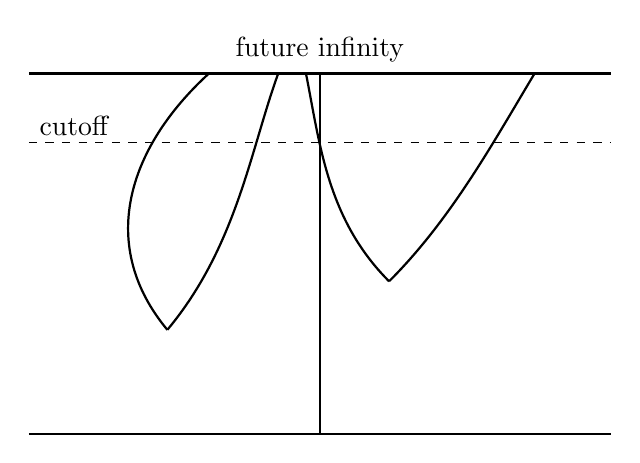
\begin{tikzpicture}[scale=0.88]
\draw[thick] (-4.2,0) -- (4.2,0);
\draw[thick] (0,0) -- (0,5.2);
\draw[thick] (-4.2,5.2) -- (4.2,5.2);
\draw[thick] (-2.2,1.5) .. controls (-3.2,2.7) and (-2.8,4.1) .. (-1.6,5.2);
\draw[thick] (-2.2,1.5) .. controls (-1.2,2.7) and (-1.0,4.1) .. (-0.6,5.2);
\draw[thick] (1.0,2.2) .. controls (0.1,3.1) and (0.0,4.2) .. (-0.2,5.2);
\draw[thick] (1.0,2.2) .. controls (1.9,3.1) and (2.5,4.2) .. (3.1,5.2);
\draw[dashed] (-4.2,4.2) -- (4.2,4.2);
\node at (0,5.55) {future infinity};
\node at (-3.55,4.45) {cutoff};
\end{tikzpicture}
\caption{Transcript-led schematic of bubble nucleation in an inflating background. The dashed line represents a cutoff. The measure problem is that bubble counts depend sensitively on how such a cutoff is imposed.}
\end{figure}

The new difficulty is not geometric but probabilistic. In an exponentially growing population, typicality arguments become treacherous. Susskind gives several examples. The cleanest abstract model is a doubling population. Then the most recent generation contains half of all observers who ever existed, the most recent two generations contain three-quarters, and the most recent three contain seven-eighths. In the idealized model,
\begin{equation}
f_{\text{last }n\text{ generations}}=1-2^{-n}.
\end{equation}
This is the mathematics behind his repeated fractions \(1/2\), \(3/4\), and \(7/8\).

He then translates the same idea into Escher's devils near the boundary of a finite drawing. It also reappears in eternal inflation. No matter how late the cutoff is imposed, a large fraction of the total count sits near the cutoff. Worse, answers to apparently simple probability questions depend sensitively on how one chooses that cutoff. That is the measure problem. In a world with exponentially increasing populations, probability assignments become hypersensitive to the details of how one truncates the infinite set before counting.

The lecture briefly pushes this picture back toward observation. Bubble collisions, if visible, could leave signatures on the microwave sky, such as unusual cold spots and characteristic polarization patterns. Susskind treats this as an open possibility rather than an established fact. The important point for the lecture is that if such evidence ever became convincing, the measure problem would stop being an abstract nuisance and become an immediate obstacle to prediction.

The lecture ends with a short coda on string theory. Susskind distinguishes the mathematically precise, supersymmetric theory, what he informally calls string theory with a capital S, from any larger structure that might describe the actual nonsupersymmetric world. The rigorous theory is internally consistent and contains gravity and quantum mechanics, but it is not the observed world. If the real world is connected to it, that connection lies in a larger and less controlled framework. The coda is therefore not a new mathematical development. It is a remark about the limits of present exact knowledge.

\section{Summary}

The lecture begins from a student's objection and builds outward without losing that opening motivation. Horizons are locally hot, and the concrete meaning of that statement is the thermometer law \(T_{\text{local}}\sim 1/(2\pi d_{\text{hor}})\). Redshift then explains why the far-away or central observer sees a much colder temperature. The same logic that organizes the black-hole case leads, in de Sitter space, to the conformal diagram, the constant horizon distance \(1/H\), and the static patch metric. A student-driven Newtonian exercise then models vacuum energy by a repulsive quadratic potential, clarifying both accelerated expansion and the huge redshift from the horizon. Once the causal patch is recognized as a finite-entropy thermal system, the lecture naturally opens into recurrence times, rare fluctuations, Boltzmann brains, eternal inflation, and the cutoff-sensitive measure problem. The chapter is therefore unified by one idea: horizon thermodynamics, once taken seriously, does not stop at radiation. It continues all the way into cosmological probability.